\documentclass[11pt,aspectratio=169]{beamer}
\usetheme{Boadilla}
\usecolortheme{beaver}
\usepackage[utf8]{inputenc}
\usepackage{amsmath}
\usepackage{amsfonts}
\usepackage{amssymb}
\usepackage[spanish,mexico]{babel}
\usepackage{graphicx}
\usepackage{multicol}

% \usepackage{ucs}
% \usepackage{beamerthemeboxes}
% \usepackage{caption}
% \usepackage{mathpazo}
% \usepackage{fontenc}
% \usepackage{booktabs}
% \usepackage{listings}
% \usepackage{algorithm,algorithmic}

\date{\today}
\author{Dr. Héctor Selley}
\institute{Universidad Anáhuac México} 
\title[Introducción a la IA]{Introducción a la Inteligencia Artificial}


\begin{document}

\AtBeginSection[] % Do nothing for \section*
{
\begin{frame}<beamer>
\frametitle{Contenido}
\tableofcontents[currentsection]
\end{frame}
}

% Título
\begin{frame}
    \titlepage
\end{frame}

% Índice
\begin{frame}
    \tableofcontents
\end{frame}

% ¿Qué es la IA?
\section{¿Qué es la IA?}
\begin{frame}{¿Qué es la IA?}
    \begin{block}{Inteligencia artificial}\pause
        La IA es un campo de estudio de las ciencias de 
        la computación que se ocupa de crear sistemas y programas capaces de 
        realizar tareas que normalmente requieren de la inteligencia humana. \pause
        El objetivo de la IA es desarrollar máquinas y sistemas que puedan 
        simular y emular la capacidad de percepción, razonamiento, aprendizaje 
        y toma de decisiones propias de los seres humanos.
    \end{block}
\end{frame}

\begin{frame}{¿Qué es la IA?}
    \begin{figure}
        \centering
        \includegraphics[scale=0.35]{"../Programacion para ML/Contenido/img/ML-multi.png"}
    \end{figure}
\end{frame}

\begin{frame}{¿Qué es la IA?}
    \begin{itemize}
        \item La IA se divide en diferentes ramas, como el aprendizaje automático 
            (machine learning), el procesamiento del lenguaje natural, la visión artificial, 
            los sistemas expertos, entre otros.\pause
        \item La inteligencia artificial se basa en algoritmos y modelos matemáticos \pause
            que permiten a las máquinas procesar grandes cantidades de datos, aprender 
            de ellos y tomar decisiones o realizar acciones en base a ese conocimiento. \pause
        \item En informática, la inteligencia expresada por máquinas, sus procesadores y 
            su software, que serían los análogos al cuerpo, el cerebro y la mente, 
            respectivamente, a diferencia de la inteligencia natural demostrada por humanos 
            y ciertos animales con cerebros complejos.\pause
	    \item En ciencias de la computación, una máquina \textit{inteligente} ideal es un 
            agente flexible que percibe su entorno y lleva a cabo acciones que maximicen 
            sus posibilidades de éxito en algún objetivo o tarea.\pause
        \item La inteligencia artificial no tiene como finalidad reemplazar a los humanos, 
            sino mejorar significativamente las capacidades y contribuciones de estos.  
    \end{itemize}
\end{frame}

\begin{frame}{¿Cómo surgió la IA?}\pause
    \begin{itemize}
        \item En 1956, John McCarthy acuñó\footnote{Acuñar: Dar forma a expresiones o 
            conceptos, especialmente cuando logran difusión o permanencia.} la expresión 
            \textit{inteligencia artificial}, y la definió como \textit{la ciencia e ingenio 
            de hacer máquinas inteligentes, especialmente programas de cómputo inteligentes}.
            \pause
        \item Se hizo presente poco después de la Segunda Guerra Mundial con el desarrollo 
            de la \textit{prueba de Turing}, mientras que la locución fue acuñada 
            por el informático John McCarthy en la Conferencia de Dartmouth. 
    \end{itemize}
\end{frame}

\begin{frame}{Prueba de Turing}
    \begin{figure}
        \centering
        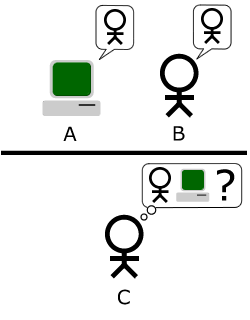
\includegraphics[scale=0.75]{img/Turing_Test_version_3.png}
    \end{figure}
\end{frame}

\begin{frame}{Prueba de Turing}
        \begin{itemize}
            \item Introducida por Alan Turing en 1950\cite{turing1} \pause 
            \item Turing plantea la pregunta: ¿Una máquina puede ganar 
                \textit{El juego de la imitación}?\pause
            \item ¿Qué es el juego de la imitación y como se juega?:\pause 
                \begin{itemize}
                    \item Tres jugadores por turnos \pause
                    \item El jugador A es hombre, B es mujer y C es el interrogador \pause
                    \item C no puede ver a los jugadores A y B (los conoce como X y Y). \pause
                    \item C se comunica con A y B mediante notas escritas, las cuales no deben
                        revelar el género.\pause
                    \item Mediante las preguntas, C debe determinar cual es el hombre
                        y cual es la mujer. \pause
                    \item El rol de A es llevar al interrogador a tomar la decisión \textbf{incorrecta}.\pause
                    \item El rol de B es ayudar al interrogador a tomar la decisión \textbf{correcta}.
                \end{itemize}
        \end{itemize}
\end{frame}

\begin{frame}{Prueba de Turing}
        \begin{itemize}
            \item Turing propone una variación: \pause 
            \item Tres participantes se encuentran en cuartos aislados: \pause
                \begin{itemize}
                    \item Una computadora (el sujeto de prueba)\pause
                    \item Un humano \pause 
                    \item Un juez (otro humano) \pause
                \end{itemize}
            \item El juez puede conversar tanto con el ordenador como con el humano mediante escritura 
                en una terminal. \pause
            \item Tanto la computadora como el jugador B tratarán de convencer al juez de que son 
                humanos.\pause
            \item El objetivo del interrogador no es determinar cuál de ellos es hombre y cual mujer sino 
                cual es computadora y cual humano. 
        \end{itemize}
\end{frame}

\begin{frame}{Prueba de Turing}
    \begin{figure}
        \centering
        \href{https://upload.wikimedia.org/wikipedia/commons/3/30/Turing-test.gif}{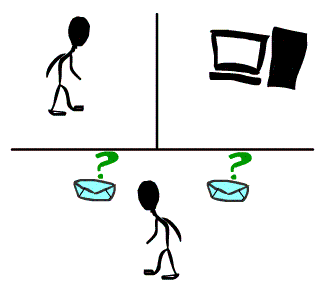
\includegraphics[scale=0.75]{img/Turing-test.png}}
    \end{figure}
\end{frame}

\begin{frame}{Prueba de Turing}
    \begin{itemize}
        \item Como señala Stevan Harnad\cite{harnad1} la pregunta se ha convertido en 
            "\textit{¿Pueden las máquinas hacer lo que nosotros (como entidades pensantes) 
            podemos hacer?}" \pause
        \item En otras palabras, Turing ya no se pregunta si una máquina puede pensar
        \item Él se pregunta si una máquina puede actuar indistintamente\cite{harnad2} a la forma 
            como lo hace un pensador. La pregunta evita el problema filosófico de definir el verbo 
            pensar y se enfoca en evaluar las capacidades que el pensar hace posible.
    \end{itemize}
\end{frame}

\begin{frame}{Prueba de Turing}
    \begin{itemize}
        \item Varios han interpretado la pregunta de Turing como: \pause
        \item \textit{¿Puede una computadora, al comunicarse a través de una terminal, engañar 
            a una persona de que es humana?} \pause 
        \item Sin embargo Turing no hablaba de engañar personas, sino de generar capacidades 
            cognitivas.\cite{harnad3}
    \end{itemize}
\end{frame}


\begin{frame}{¿Qué es la IA?}
    John Searle introdujo una distinción entre los tipos de IA\pause \cite{searle}:
    \begin{itemize}
        \item IA fuerte \pause
        \item IA débil
    \end{itemize}
\end{frame}

\begin{frame}{¿Qué es la IA?}
    \begin{block}{IA fuerte}\pause
        La IA es la ciencia e ingeniería que permtirá replicar la inteligencia
        humana mediante máquinas.
    \end{block}\pause
    También conocida como \textbf{dura}, en ella se busca construir máquinas que
    razonen como lo hacen los humanos, este es el campo de trabajo de neurobiólogos
    y neurocientíficos, falta mucho por hacer.
\end{frame}

\begin{frame}{¿Qué es la IA?}
    \begin{block}{IA débil}\pause
        La IA es la ciencia e ingeniería que permite diseñar y programar
        ordenadores de forma que realicen tareas que requieren inteligencia.
    \end{block}\pause
    El objetivo no es reproducir exactamente los procesos de pensamiento humano,
    sino conseguir que las máquinas sean capaces de resolver problemas como lo 
    hacen las personas o inclusive mejor, en un dominio restringido.
\end{frame}

\begin{frame}{Tipos de IA}
    Stuart J. Russell y Peter Norvig diferencian varios tipos de inteligencia artificial:
    \begin{description}
        \item[Sistemas que piensan como humanos] Estos sistemas tratan de emular el pensamiento humano; por ejemplo, las redes neuronales artificiales. La automatización de actividades que vinculamos con procesos de pensamiento humano, actividades como la toma de decisiones, resolución de problemas y aprendizaje.       
        \item[Los sistemas que actúan como humanos] Estos sistemas tratan de actuar como humanos; es decir, imitan el comportamiento humano; por ejemplo, la robótica (El estudio de cómo lograr que los computadores realicen tareas que, por el momento, los humanos hacen mejor).
    \end{description}
\end{frame}

\begin{frame}{Tipos de IA}
    \begin{description}
        \item[Los sistemas que piensan racionalmente] Es decir, con lógica (idealmente), tratan de imitar el pensamiento racional del ser humano; por ejemplo, los sistemas expertos, (el estudio de los cálculos que hacen posible percibir, razonar y actuar).
        \item[Los sistemas que actúan racionalmente] Tratan de emular de forma racional el comportamiento humano; por ejemplo, los agentes inteligentes, que está relacionado con conductas inteligentes en artefactos.
    \end{description}
\end{frame}

% Historia
\section{Historia}
\begin{frame}{Historia}
    \begin{figure}
        \centering
        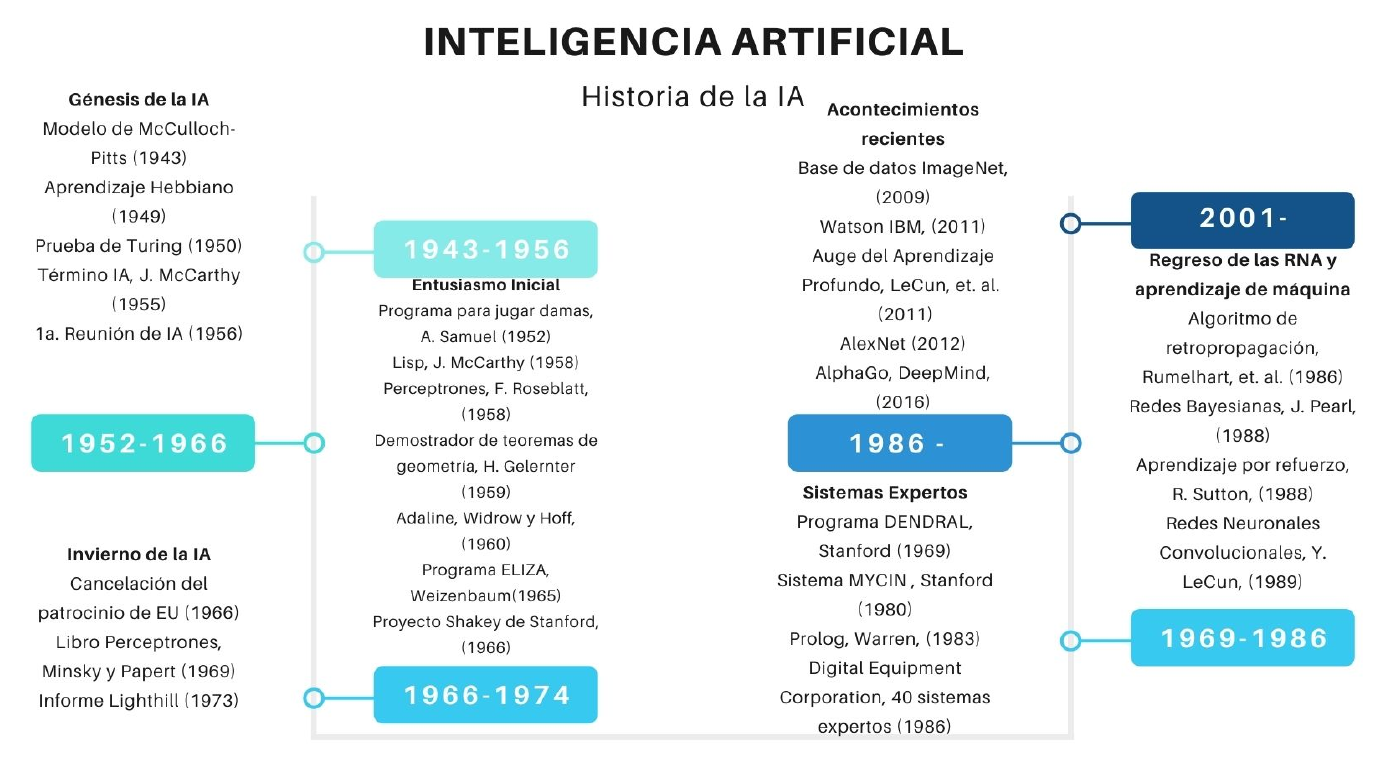
\includegraphics[scale=0.35]{img/historiaIA.png}
    \end{figure}
\end{frame}

\begin{frame}{Historia}
    \begin{figure}
        \centering
        \includegraphics[scale=0.35]{"../Programacion para ML/Contenido/img/AI-ML2.png"}
    \end{figure}
\end{frame}

% Aplicaciones
\section{¿Para qué sirve la IA?}
\begin{frame}{Aplicaciones}
    \begin{itemize}
        \item Lingüística computacional\pause
        \item Minería de datos (Data Mining)\pause
        \item Industria\pause
        \item Medicina\pause
        \item Mundos virtuales\pause
        \item Procesamiento de lenguaje natural (Natural Language Processing)\pause
        \item Robótica\pause
        \item Sistemas de control
    \end{itemize}
\end{frame}

\begin{frame}{Aplicaciones}
    \begin{itemize}
        \item Sistemas de apoyo a la decisión\pause
        \item Videojuegos\pause
        \item Prototipos informáticos\pause
        \item Análisis de sistemas dinámicos\pause
        \item Simulación de multitudes\pause
        \item Sistemas Operativos\pause
        \item Automoción
    \end{itemize}
\end{frame}


\begin{frame}{Ejemplos:}
    \begin{itemize}
        \item \textbf{Asistentes de voz}. 
            Máquinas que utilizan el procesamiento de lenguajes naturales para interpretar qué es lo que se les está comunicando 
            y, de este modo, poder responder a las necesidades humanas, ya sea verbalmente o mediante la ejecución de una acción concreta. \pause
        
        \item \textbf{Smartphones}.
            Poseen un asistente de voz per van mucho más allá, y está presente en multitud de acciones que ni siquiera percibimos. Por ejemplo, cuando 
            seleccionamos el modo retrato de la cámara de fotos y es el propio smartphone el que arregla la foto de manera automática para que salgamos 
            lo más favorecidos posible. Eso también es gracias a la inteligencia artificial. \pause
    \end{itemize}
\end{frame}
    
\begin{frame}{Ejemplos:$_2$}
    \begin{itemize}
        \item \textbf{Análisis de hábitos}.
            Análisis de los datos que producimos de forma continua y que permiten conocer nuestros hábitos. Gracias a la combinación de Big Data 
            e inteligencia artificial, se pueden analizar 	los hábitos de consumo de cada persona, lo que también ofrece ventajas muy interesantes. Gracias 
            a esto se puede ofrecer contenido personalizado (publicidad que recibe cada usuario). Pero también 
            es fundamental a la hora de luchar contra el fraude digital, por ejemplo en el sector bancario, financiero o de las aseguradoras. 
            
        \item \textbf{Aplicaciones médicas}.
            Gracias a la inteligencia artificial, las máquinas trabajan mano a mano con los doctores y cirujanos. Estas máquinas están programadas para llegar
            a donde el ojo clínico del médico no consigue hacerlo. De esta forma, tenemos desfibriladores, máquinas quirúrgicas y máquinas de diagnóstico que 
            se valen de una IA para ofrecer mejores resultados. 
    \end{itemize}
\end{frame}
    
\begin{frame}{Ejemplos:$_3$}
    \begin{itemize}
        \item \textbf{Optimización de rutas}.
            Estas inteligencias artificiales nos ofrecen la mejor alternativa para realizar los desplazamientos a partir de la 
            comparación de multitud de datos, desde datos geográficos a datos relativos a la situación actual del entorno en el que nos desplazamos (por ejemplo, 
            condiciones meteorológicas o información relativa al tráfico). De hecho, gracias a aplicaciones como PlannerPro by Beetrack, se pueden planificar y 
            diseñar las rutas de reparto de la manera más eficiente posible, garantizando la optimización de los recursos disponibles y ofreciendo la mejor calidad 
            de servicio a los clientes. 
    \end{itemize}
\end{frame}

\begin{frame}{Aplicaciones}
    \begin{figure}
        \centering
        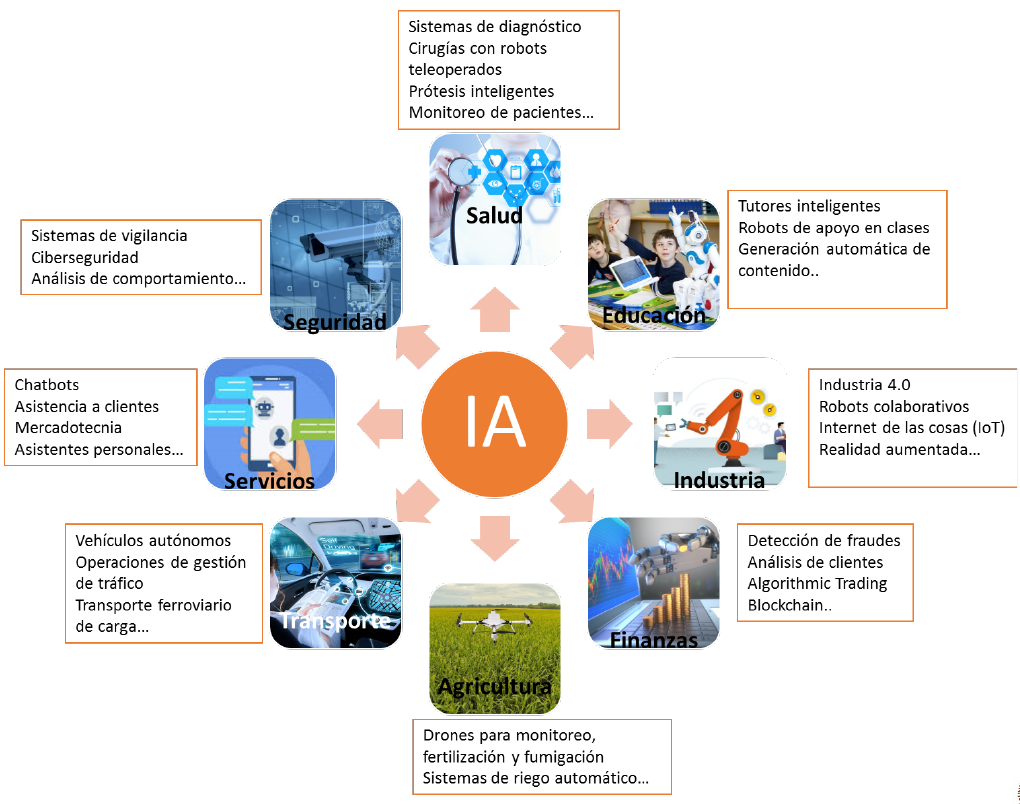
\includegraphics[scale=0.35]{img/aplicacionesIA.png}
    \end{figure}
\end{frame}

\begin{frame}{Tesis de doctorante}
    \begin{block}{Tema}
        Redes neuronales recurrentes para la interpretación de laLengua de Señas Mexicana (LSM) 
        en servicios de salud a través de Inteligencia Artificial
    \end{block}     
    \begin{figure}
        \centering
        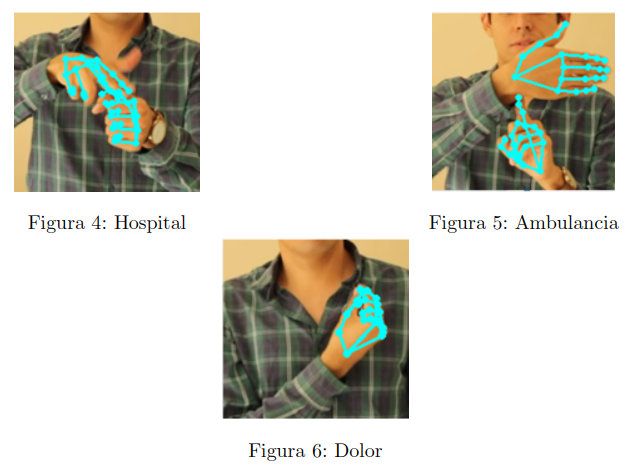
\includegraphics[scale=0.45]{img/LenguajeSenas.png}
    \end{figure}
\end{frame}

\begin{frame}{Paradigma}
    \begin{figure}
        \centering 
        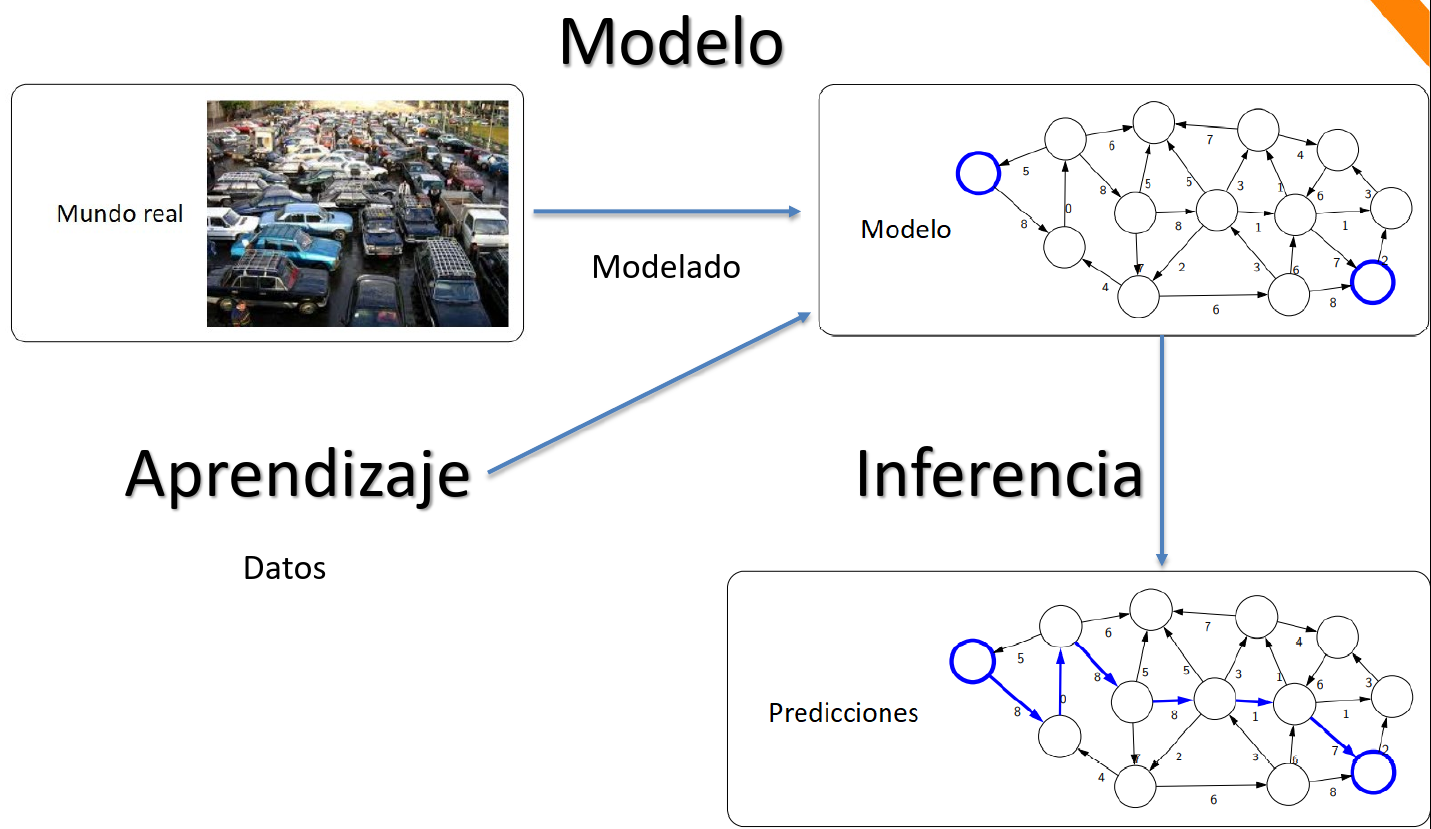
\includegraphics[scale=0.25]{img/paradigma.png}
    \end{figure}
\end{frame}


\section[Ética]{Dilemas éticos}
\subsection{Privacidad}
\begin{frame}{Privacidad}
    \begin{figure}
        \centering
        \includegraphics[scale=0.5]{"../Programacion para ML/Contenido/img/ads.jpg"}
    \end{figure}
\end{frame}

\begin{frame}{Privacidad}
    \begin{figure}
        \centering
        \href{https://www.businessinsider.com/the-incredible-story-of-how-target-exposed-a-teen-girls-pregnancy-2012-2?r=MX&IR=T}{\includegraphics[scale=0.27]{"../Programacion para ML/Contenido/img/target.png"}}
    \end{figure}
\end{frame}

\begin{frame}{Privacidad y seguridad de los datos}
    \begin{block}{Privacidad}
    Es un derecho humano intrínseco, que muchas personas desconocen, no ejercen o incluso renuncian a el. Sin embargo, la 
    privacidad no es un tema menor y en la actualidad debe preocuparnos por lo menos conocer ese derecho.
    \end{block}
\end{frame}
    
\begin{frame}{Privacidad y seguridad de los datos}
    \begin{itemize}
        \item Conforme el Internet de las cosas crezca, será cada vez más difícil preservar la privacidad. \pause
        \item Smartphone (sensores)
            \begin{itemize}
                \item Acelerómetro\pause
                \item Barómetro\pause
                \item Capacitivos\pause
                \item Giroscopio\pause
                \item GPS\pause
                \item Huella dactilar\pause
                \item Iris\pause
                \item Podómetro\pause
                \item Magnetómetro (brújula electrónica)\pause
                \item Proximidad\pause
                \item Luz ambiental\pause
                \item Espectro de color\pause
                \item Ritmo cardiaco\pause
                \item Infrarrojo
            \end{itemize}
    \end{itemize}
\end{frame}
    
\begin{frame}{Privacidad y seguridad de los datos}
    \begin{itemize}
        \item Si un usuario no conoce la política de uso de estos datos por parte del fabricante, concede libertad completa del uso de dichos datos.\pause
        \item Por otro lado, si un usuario desea leer la política de uso de datos de algún fabricante, esta no será fácilmente comprensible. \pause
            \begin{itemize}
                \item Tecnicismos\pause
                \item Redacción deliberadamente confusa\pause
            \end{itemize}
        \item En ocasiones no sólo se trata de desconocimiento o apatía del usuario, puede ser el caso de que un fabricante o proveedor no le facilite la tarea.
    
    \end{itemize}
\end{frame}

\begin{frame}{Redes sociales}
    \begin{itemize}
        \item Es posible que Facebook conozca mucho de una persona que no tenga una cuenta en su servicio.\pause
        \item Personas alrededor tienen una cuenta activa\pause
        \item Suban fotografías en las que la primer persona se encuentre\pause
        \item Ahora Facebook sabe que existes. 
    \end{itemize}
    \end{frame}
    
    \begin{frame}{Privacidad}
    \begin{block}{}
        \begin{center}
            El principal obstáculo de la privacidad consiste en que los consumidores desconozcan que se estén recolectando datos acerca de el sin su consentimiento.
        \end{center}	
    \end{block}
    \end{frame}
    
    \begin{frame}{Privacidad}
    \begin{itemize}
        \item Las compañías que basan su modelo de negocios en la recolección de datos y publicidad dirigida no quieren cambios.\pause
        \item Favorecer la privacidad del usuario va en contra de su negocio.\pause
        \item Sería como pedirle a Spotify o Youtube que ponga en silencio automáticamente los anuncios de su plataforma.
    \end{itemize}
    \end{frame}
    
    \begin{frame}{Privacidad}
    En su reporte anual del 2014, Google identificó como un riesgo las tecnologías que bloquean anuncios automáticamente:\pause
    \begin{block}{}
    \textit{Existen tecnologías y herramientas que han sido desarrolladas para bloquear nuestros anuncios y permitir a los usuarios no verlos. La mayoría 
    de nuestras ganancias provienen de las cuotas que nos pagan compañías por mostrar sus anuncios en nuestras páginas para los usuarios. Como consecuencia, 
    estas tecnologías y herramientas afectan nuestros resultados operativos.}
    \end{block}
    \end{frame}
    
    \begin{frame}{Privacidad}
    \begin{itemize}
        \item Facebook está en la misma sintonía. \pause
        \item Sus ingresos por publicidad por año representan:\item 
            \begin{itemize}
                \item 2012 $\Rightarrow$ 84\% \pause
                \item 2013 $\Rightarrow$ 89\% \pause
                \item 2014 $\Rightarrow$ 92\%
            \end{itemize}
    \end{itemize} 
    \end{frame}
    
    \begin{frame}{Privacidad}
    \begin{itemize}
        \item Cuando los usuarios borran las \textit{cookies} o utilizan un programa que bloquea los anuncios, afecta al modelo de negocios de compañías que 
        venden el despliegue de anuncios. \pause
        \item Coupons.com advierte a sus inversionistas:\pause
    \end{itemize}
    \begin{block}{}
        \textit{... el navegador Safari bloquea las cookies de terceros por defecto, y los desarrolladores de Firefox anunciaron que sus futuras versiones 
        del navegador harán lo mismo. A menos que estas configuraciones sean modificadas directamente por los usuarios, no nos será posible almacenar 
        la misma cantidad de cookies lo que afectará directamente a nuestro modelo de negocio.}
    \end{block}\pause
    \begin{itemize}
        \item La tecnología en este aspecto está protegiendo la privacidad de los usuarios.\pause
        \item Debe estar en desarrollo algún tipo distinto de tecnología/estrategia que les permita seguir obteniendo datos de sus usuarios.
    \end{itemize}	
    \end{frame}

\subsection{Regulación}
\begin{frame}{Regulación}
    \begin{itemize}
        \item En marzo de 2023, cientos de empresarios como Elon Musk, Steve Wozniak 
            (cofundador de Apple) o los presidentes de numerosas compañías tecnológicas; 
        \item intelectuales como Yuval Noah Harari y cientos de académicos e investigadores 
            especializados en inteligencia artificial firmaron una carta abierta avisando 
            del peligro de la falta de regulación de la IA, 
        \item Ponen el foco sobre OpenAI, la empresa que ha desarrollado ChatGPT. 
        \item Pidieron una pausa de al menos 6 meses para sus experimentos más potentes, 
            hasta que el mundo logre un consenso internacional para que estos sistemas 
            «sean más precisos, seguros, interpretables, transparentes, robustos, neutrales, 
            confiables y leales».
    \end{itemize}
\end{frame}

\begin{frame}{Regulación}
    \begin{figure}
        \centering
        \href{https://www.eldiario.es/tecnologia/creadores-inteligencias-artificiales-academicos-piden-equiparar-riesgos-bomba-nuclear_1_10253632.html}{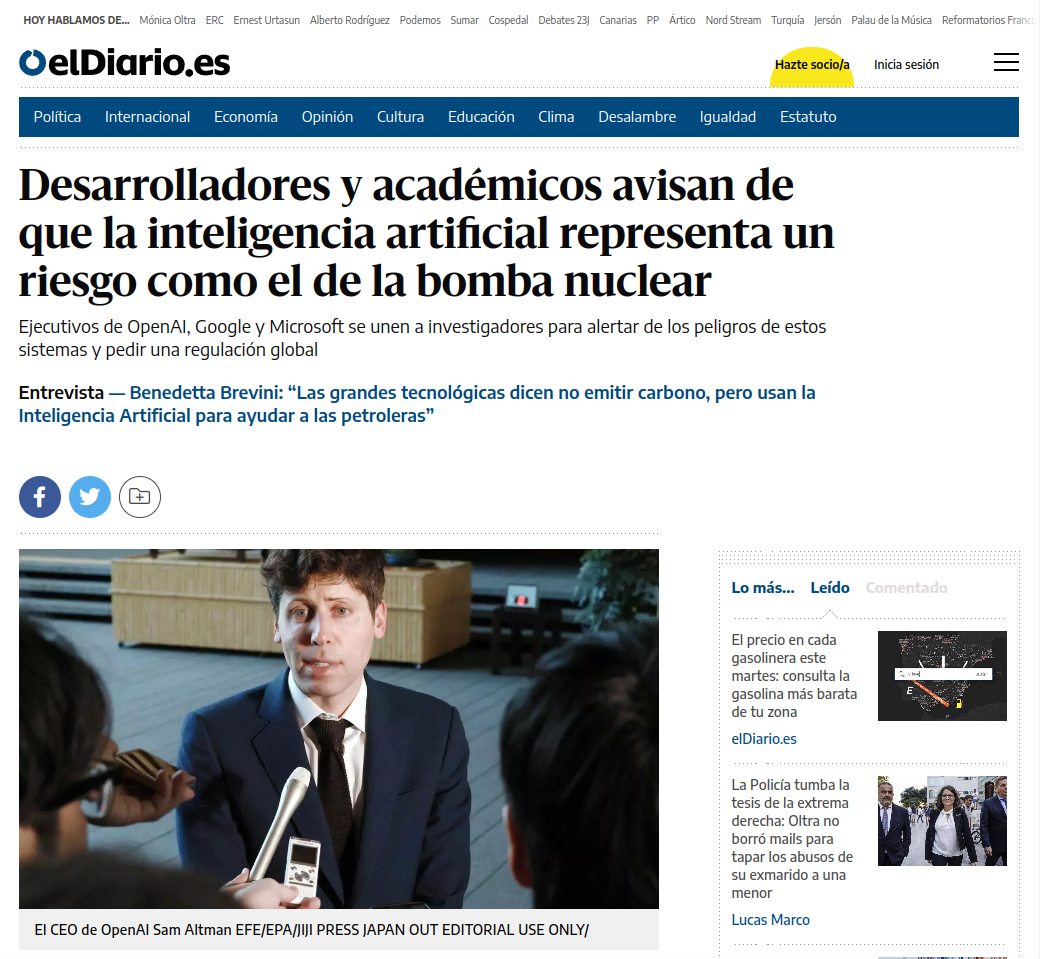
\includegraphics[scale=0.35]{img/RiesgoIAmayo2023.png}}
    \end{figure}
\end{frame}

\begin{frame}{Regulación}
    \begin{itemize}
        \item Dos meses más tarde, en mayo, 350 ejecutivos de las principales empresas 
            desarrolladoras de IA, académicos e investigadores expertos firmaron un nuevo 
            manifiesto \pause
        \item En este manifiesto alertan que la IA avanzada sin regular representa un peligro de 
            extinción para la humanidad: \pause
    \end{itemize}
    \begin{block}{Manifiesto}
        \textit{Mitigar el riesgo de extinción de la IA debería ser una prioridad mundial junto a otros riesgos a escala social como las pandemias y la guerra nuclear}
    \end{block}
\end{frame}

\begin{frame}{Regulación}
    Entre los impulsores de esta petición están:
    \begin{itemize}
        \item Toda la plana mayor de OpenAI \pause
        \item El jefe de Tecnología de Microsoft \pause
        \item El líder de Google DeepMind \pause
        \item 38 ejecutivos, investigadores o profesores de universidad relacionados con la empresa\pause
        \item Representantes de desarrolladoras más pequeñas como Anthropic, Stability AI o Inflection AI.
    \end{itemize}
\end{frame}


\section{Bibliografía}
\begin{frame}[allowframebreaks]{References}
    \nocite{*}
    \bibliographystyle{plain}
    \bibliography{biblioIA}
\end{frame}
\end{document}

